\section{Moduł WAVES}

\subsection{Badania literaturowe}

Celem niniejszej pracy było zaimplementowanie oraz przetestowanie działania algorytmu  detekcji punktów charakterystycznych syganłu EKG. W tym początku i końca zespołu QRS (QRS-onset i QRS-end) oraz fali P (P-onset i P-end). Numery próbek załamków R przyjmowane są  jako dane wejściowe wraz z przefiltrowanym sygnałem. Graficznie opisywane punkty przedstawione zostały na rysunku ~\ref{fig:Waves_EKG}.


\begin{figure}[h]
\centering
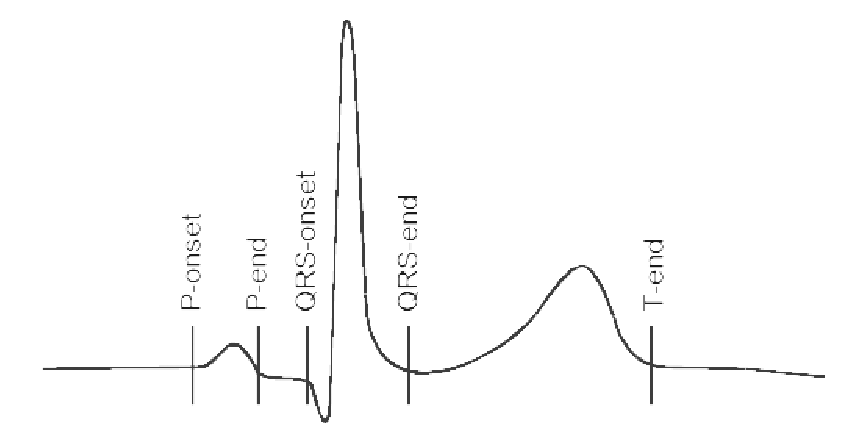
\includegraphics[width=\textwidth,keepaspectratio] {Waves/img/EKG_pts.eps}
\caption{Sygnał EKG z punktami charakterystycznymi. Źródło: \cite{Waves_PSED}}
\label{fig:Waves_EKG}
\end{figure}

Zespół QRS jest fragmentem zapisu elektrokardiograficznego odpowiadającego depolaryzacji, czyli pobudzeniu prawej i lewej komory serca. Czas jego trwania oraz kształt niosą wiele informacji na temat aktualnej kondycji serca. Dzięki swojemu charakterystycznemu kształtowi oraz wysokiej energii stanowi on często podstawę wszystkich automatycznych systemów analizy sygnałów EKG. 
Mimo intensywnych prac na przestrzeni przeszło trzydziestu lat programowe wyznaczanie zespołu QRS wciąż stanowi wyzwanie dla projektantów. Bardzo duże zróżnicowanie morfologiczne analizowanych sygnałów powoduje, że do tej pory nie opracowano detektora działającego ze stu procentową dokładnością. W ostatnich latach dynamiczny rozwój techniki pozwolił na stosowanie czasochłonnych algorytmów o dużej złożoności obliczeniowej (wyjątkiem są tu urządzenia przenośne, ze względów na bateryjne zasilanie). Zaowocowało to szeregiem nowych podejść do problemu detekcji punktów charakterystycznych zespołu QRS. W literaturze odnaleźć można algorytmy oparte o sztuczne sieci neuronowe, algorytmy genetyczne, przekształcenia falkowe, banki filtrów cyfrowych, ukryte modele Markowa, transformatę Hilberta oraz heurystyczne metody, w większości oparte o nieliniowe przekształcenia \cite{Waves_TPoSQD} \cite{Waves_Pieciak}. Cechą wspólną niemal wszystkich rozwiązań jest odpowiednie przygotowanie próbek sygnału do analizy, czyli filtracja sygnału mająca na celu usunięcie zakłóceń mięśniowych, sieciowych 50/60 Hz, zmiennej impedancji elektrod oraz artefaktów powstałych wskutek ruchu pacjentów podczas badania.
Fala P odpowiada natomiast depolaryzacji przedsionków serca i w warunkach prawidłowych występuje na schemacie zapisu elektrokardiograficznego przed zespołem QRS. Stanowi ona logiczny początek pojedynczego cyklu pracy serca. Jak w przypadku zespołu QRS automatyczne wyznaczanie początku i końca fali P cieszy się wśród projektantów dużym zainteresowaniem. Podobnie nie stworzono wciąż bezbłędnego algorytmu detekcji, gdyż wykrywanie załamka P nie jest zadaniem prostym. Ma na to wpływ parę czynników, z których można wymienić: zmienną amplitudę fali, możliwą interferencję z innymi falami występującymi w sygnale EKG, a nawet czasem brak występowania. W literaturze można znaleźć wiele przykładów badających problematykę znalezienia załamka P. Stosowane na świecie metody bazują na:
\begin{itemize}
\item pochodnych sygnału \cite{Waves_ANAfPDitES}
\item transformacie fazowej sygnału \cite{Waves_aNMfADoEFPBotPT}    \cite{Waves_ProjZeszlyRok}
\item filtrowaniu sygnału filtrami górnoprzepustowymi \cite{Waves_ARPfPDaSiHR12E}
\item transformacie falkowej \cite{Waves_DoCPoEUQSWT}
\end{itemize}
W zależności od wybranej metody algorytmy różnią się między sobą dokładnością jak i złożonością obliczeniową. Autorzy algorytmu bazującego na 9 punktowej pochodnej sygnału \cite{Waves_ANAfPDitES} zapewniają o skuteczności ok 90 procent, co nie jest wartością przekonującą. W przypadku zastosowania transformaty fazowej wyniki znalezione w publikacji \cite{Waves_aNMfADoEFPBotPT} są obiecujące: ponad 98\% procentowa wykrywalność oraz mała złożoność obliczeniowa. Skuteczność algorytmu mogła być ostatecznie sprawdzona podczas realizacji Projektu EKG \cite{Waves_ProjZeszlyRok} w ramach zajęć laboratoryjnych z przedmiotu Elektroniczne systemy diagnostyki medycznej i terapii w roku 2012/2013, kiedy został on zaimplementowany właśnie do wykrywania fali P. Niestety opracowane wyniki nie dają jednoznacznej odpowiedzi na pytanie co do przydatności algorytmu. Wynika to z tego, iż w pracy \cite{Waves_ProjZeszlyRok} znajdują się jedynie procentowe wykrycia ilości początków fali i końców P  w stosunku do znalezionych załamków R w sygnale. O ile w przypadku badania jakości wykrycia zespołów QRS taka metoda jest akceptowalna, to wiązanie ilości wykrytych początków i końców fali P z ilościami wykrytych załamków R jest niewłaściwe. Nie wiadomo także, czy wykryte załamki to faktycznie załamki P, czy może kawałki uchwyconego załamka T. Dlatego też, jedynym możliwym sposobem na weryfikację algorytmu jest porównanie otrzymanych punktów z wartościami referencyjnymi, którą zaproponowano w tej pracy.

\subsection{Koncepcja proponowanego rozwiązania}

\subsubsection{QRS-onset i QRS-end}

W trakcie realizacji moduły Waves, do wyznaczenia punktów charakterystycznych zespołu QRS zdecydowano się na algorytm bazujący na wyznaczaniu wskaźnika będącego wartością obszaru wyznaczonego obwiednią analizowanego zespołu. Algorytm ten, opisany szczegółowo w pracy \cite{Waves_QRSAlg} , można podzielić na cztery etapy, które zostały opisane poniżej (Detekcja załamka R opisana w pracy \cite{Waves_QRSAlg} została pominięta gdyż pozycja załamka R przyjmowana jest jako parametr wejściowy z innego modułu). 

\begin{description}
\item[Filtracja pasmowa]
Celem filtracji jest przekształcenie sygnału faworyzując cechy zespołu QRS, jednocześnie osłabiając cechy innych elementów elektrokardiogramu i zakłóceń. Częstotliwości odcięcia filtru pasmowego są odmienne dla detekcji QRS-onset i QRS-end i wynoszą odpowiednio [0.5 40] Hz oraz [5 30] Hz. Realizację filtru oparto o algorytm FFT (ang. Fast Fourier Transform). W tym celu  
wyznaczono transformatę całego sygnału, zastąpiono niechciane częstotliwości zerami, a następnie obliczono odwrotną transformatę wykorzystując algorytm IFFT (ang. Inverse Fast Fourier Transform).

\item[Wyznaczanie Obwiedni]
Obwiednia zbudowana jest z przefiltrowanego sygnału (części rzeczywistej) oraz jego przekształcenia Hilberta (części urojonej). Transformata Hilberta rzeczywistego sygnału x(t) zdefiniowana jest wzorem ~\ref{eq:Waves_HT1}.

\begin{equation} \label{eq:Waves_HT1}
x_H = \mathcal{H}\{x(t)\}=\frac{1}{\pi}\int_{-\infty}^\infty \frac{x(\lambda)d\lambda}{t-\lambda}
\end{equation}

Zamiast korzystać bezpośrednio z definicji można także wyznaczyć ją w domenie częstotliwości zgodnie z ~\ref{eq:Waves_HT2}.

\begin{equation} \label{eq:Waves_HT2}
X_H (j \omega) = X(j \omega) \cdot [-j \cdot sgn(\omega)]
\end{equation}

Następnie jeśli jako ECG oznaczymy rzeczywistą części sygnału przefiltrowanego, a jako ECGH część urojoną przekształcenia Hilberta sygnału to obwiednie możemy zdefiniować jako ~\ref{eq:Waves_ENV}.

\begin{equation} \label{eq:Waves_ENV}
ECG_{e} (k) = \sqrt{ECG^2 (k)+ ECG_{H}^2 (k) }
\end{equation}

Rysunek ~\ref{fig:Waves_ENV} pokazuje przykładowy zespół QRS wraz z wyznaczoną dla niego obwiednią . 

\begin{figure}[h]
\centering
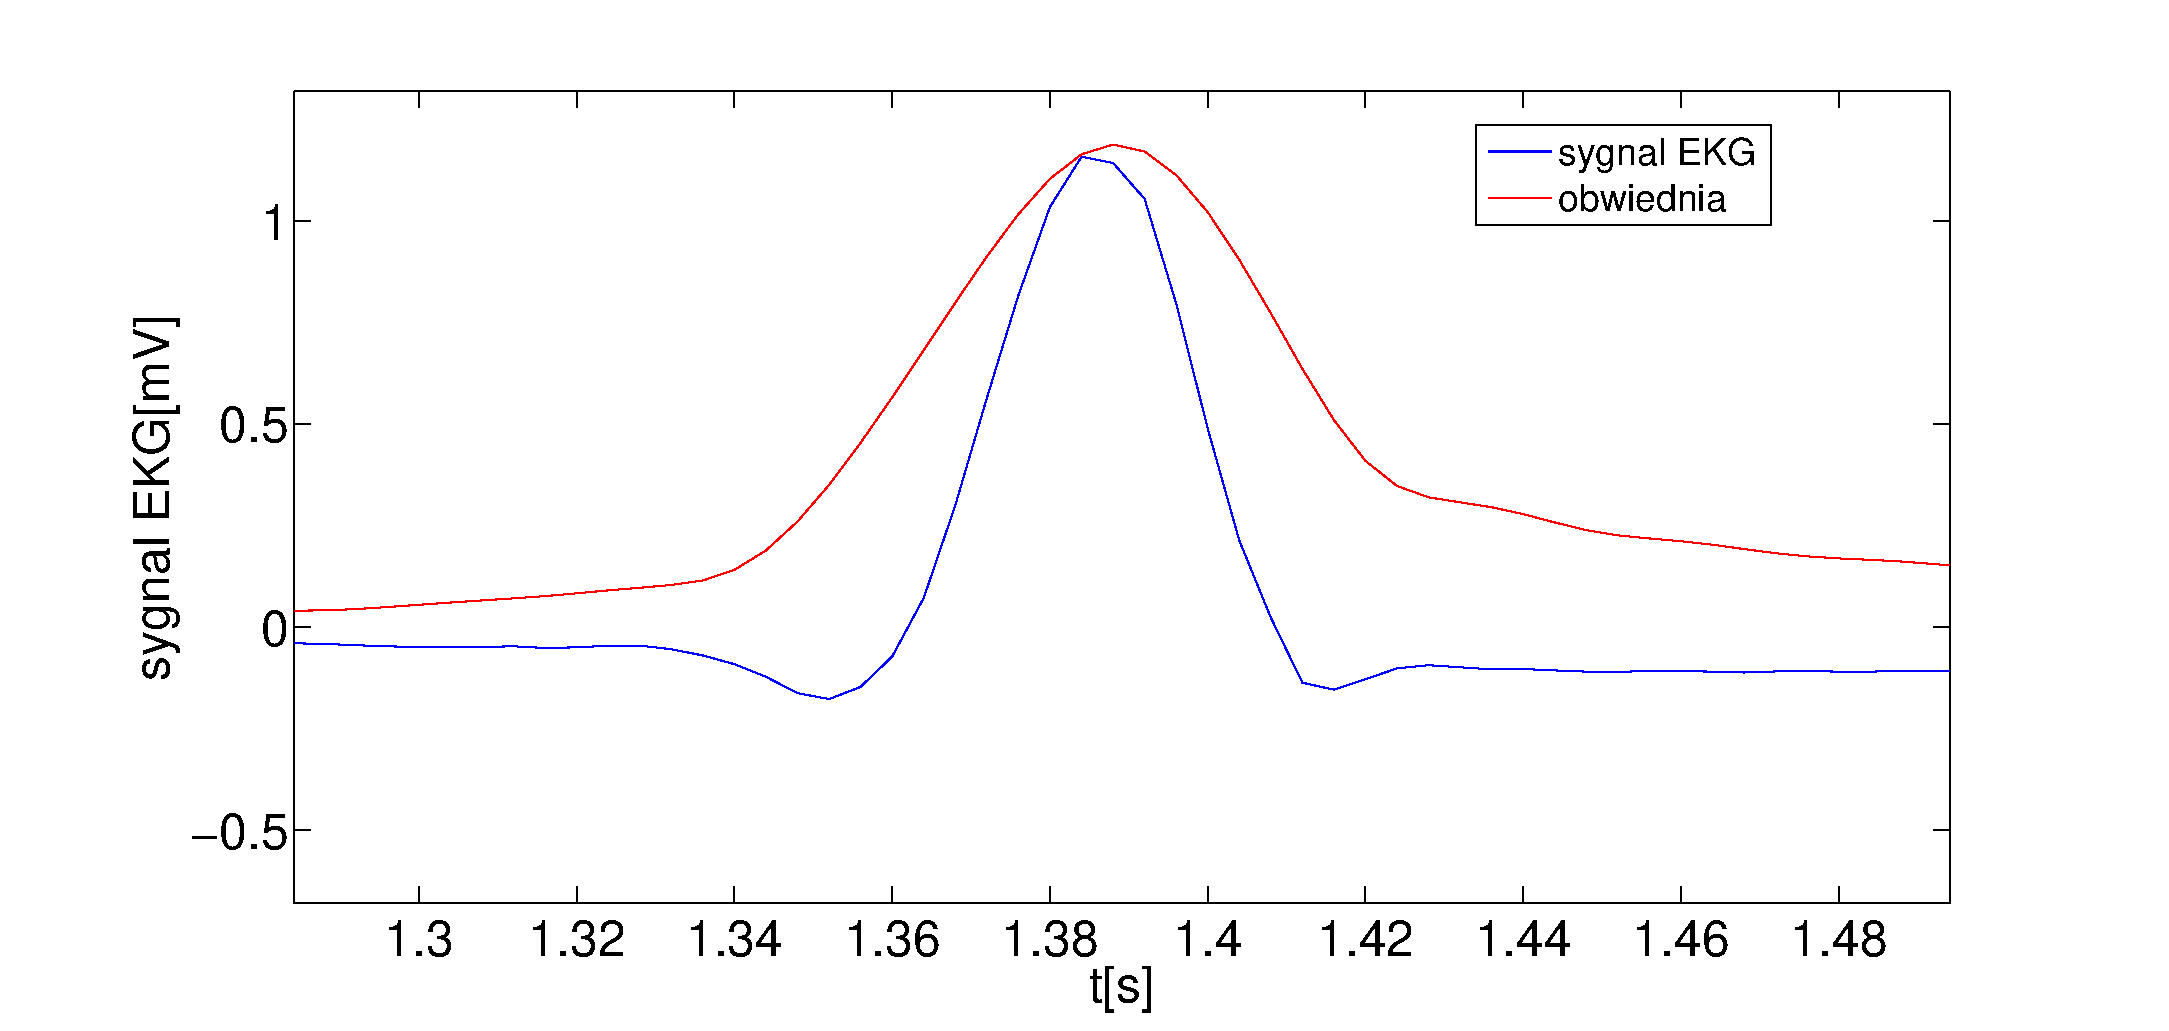
\includegraphics[scale=0.7] {Waves/img/Envelope.eps}
\caption{Sygnał EKG wraz z odpowiadającą mu obwiednią.}
\label{fig:Waves_ENV}
\end{figure}

Należy zauważyć, że wypłaszczenia obwiedni zbiegają się z początkiem i końcem zespołu QRS. Fakt ten zostanie wykorzystany w późniejszych krokach do detekcji punktów QRS-onset i QRS-end.

\item[Wyznaczanie Okna]
W celu ograniczenia zakresu poszukiwania punktów charakterystycznych zespołu QRS, zdefiniowane zostały wstępne okna w każdym cyklu pracy serca. Ze względu na czas trwania zespołu od 60 do 110 ms zdecydowano się na przeszukiwanie sygnału 100 ms przed wystąpieniem załamka R i 100 ms po nim odpowiednio dla QRS-onset i QRS-end. Taka szerokość okna powinna zapewnić objęcie pożądanych punktów, jednocześnie nie zachodząc na falę P i T. W związku z powyższym skuteczność algorytmu w sposób oczywisty zależy od poprawności wykrycia załamków R.

\item[Wyznaczanie wskaźnika powierzchni]
 Ostatnim i kluczowym krokiem algorytmu jest wyznaczenie wskaźnika powierzchni w oknie przesuwnym. Wszystkie poniższe czynności wykonywane są dla każdego cyklu serca, tylko w opisanych w poprzednim kroku oknach. Algorytm zostanie opisany na podstawie detekcji punktu QRS-end, dla ułatwienia rozpatrzony zostanie czas ciągły. Dla punktu QRS-onset postępowanie jest analogiczne i nie będzie w pracy opisane. Dla poniższych rozważań przyjęto następujące oznaczenia (patrz rysunek ~\ref{fig:Waves_A_t}):


env(t) - obwiednia sygnału w czasie, \newline
$t_1 $ i $t_2$  początek i koniec obwiedni, \newline
$t_p$ - punkt szczytowy obwiedni, \newline
$L = t_{1}-t_{2}$ - długość obwiedni pojedynczego zespołu QRS. \newline
W – szerokość okna przesuwnego

\begin{figure}[h]
\centering
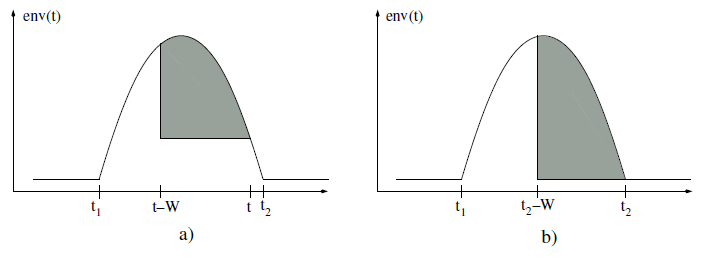
\includegraphics[width=\textwidth,keepaspectratio] {Waves/img/A_t.png}
\caption{Ilustracja wskaźnika powierzchni A(t) - szare obszary, Źródło: \cite{Waves_QRSAlg}}
\label{fig:Waves_A_t}
\end{figure}

Wykorzystany algorytm opiera się na wyznaczeniu wskaźnika A(t), który osiąga maksymalną wartość dla czasu równego $t_2$. Wyznaczany jest on przez całkowanie w oknie przesuwnym o szerokości W (wyznaczenie wartości W omówione będzie w dalszej części). W każdej chwili czasu wskaźnik może być wyliczony jako ~\ref{eq:Waves_A_t}:

\begin{equation} \label{eq:Waves_A_t}
A(t)=\int_{t-W}^t [env(\tau)-env(t)]d\tau
\end{equation}

Wskaźnik ten jest polem powierzchnią pod wykresem obwiedni w obszarze [t-W, t], ale nad poziomą linią przechodzącą przez punkt (t, env(t)). Zobrazowano to na rysunku ~\ref{fig:Waves_A_t}.
W związku z dużym zróżnicowaniem wartości L, szerokość okna W będzie osobno strojona dla każdego zespołu QRS. Jak wynika z rysunku ~\ref{fig:Waves_W0}, dla poprawnej detekcji QRS-end, wskaźnik powierzchni 2.4 powinien być wyznaczany w oknie W spełniającym zależność: $t_2 - t_p < W < L$.

\begin{figure}[h]
\centering
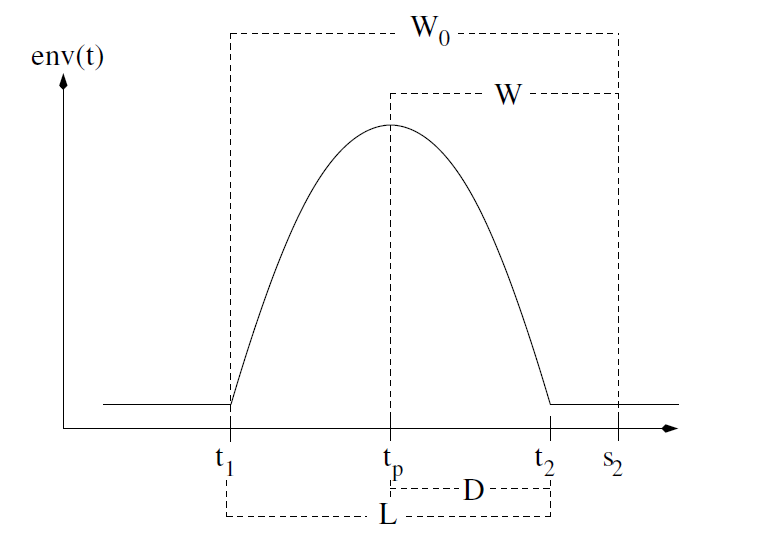
\includegraphics[width=\textwidth,keepaspectratio] {Waves/img/W0.png}
\caption{Dwuetapowy wybór okna W, Źródło: \cite{Waves_QRSAlg}}
\label{fig:Waves_W0}
\end{figure}
Kiedy wartość W jest zbyt duża, przykładowo równa $W_0$, wtedy wskaźnik przyjmuje największą wartość dla końca okna, w punkcie oznaczonym $s_2$ na rysunku ~\ref{fig:Waves_W0}. Jeśli $W_0$  nie jest zbyt duże, punkt $s_2$ powinien leżeć wystarczająco blisko $t_2$ aby spełniać warunek $s_2 - t_p < L$. W związku z tym brana jest wartości szerokości okna równa $W = s_2 - t_p$ i powtórnie wyznaczany jest wskaźnik A(t).
Podsumowując powyższe rozważania krok algorytmu można podzielić na dwie fazy: \newline
1. Obliczenie wskaźnika powierzchni dla okna przesuwnego $W=W_0$, gdzie $W_0$ jest szerokością okna opisaną w poprzednim kroku (100 ms). Wyznaczenie wartości $s_2$ maksymalizującej wskaźnik A(t) oraz wartości tp będącej maksimum obwiedni w oknie $W_0$. \newline
2. Ponowne obliczenie wskaźnika powierzchni dla okna przesuwnego o szerokości $W= s_2 - t_p$. Punkt QRS-end jest punktem maksymalizującym wskaźnik A(t).
\end{description}

\subsubsection{P-onset i P-end}
Brak rzetelnej oceny we wcześniej pracy \cite{Waves_ProjZeszlyRok} spowodował, że podjęto decyzję o ponownej implementacji algorytmu wykrywania fali P za pomocą transformaty fazowej i poprawnej weryfikacji jego skuteczności. Szczegółowe informacje co do metody można znaleźć w publikacji \cite{Waves_aNMfADoEFPBotPT}
Transformata fazowa sygnału polega na zamienieniu próbki EKG we wskaz w płaszczyźnie zespolonej wg wzoru ~\ref{eq:Waves_yN}:

\begin{equation} \label{eq:Waves_yN}
y[n]=Rv+j \cdot x[n], dla n=1,2...,N
\end{equation}

Sygnał po transformacie składa się zatem ze rzeczywistej stałej części Rv i urojonej części x[n], będącą wartością sygnału w próbce n. Moduł i faza wskazu jest obliczany jako: \newline
$M[n]=\sqrt{Rv^2+x[n]^2}$ \newline
$\phi [n]= arctan(\frac{x[n]}{Rv})$ \newline
Wykrywanie fali P dokonuje się na podstawie badania wartości fazy $\phi$, obliczanej w odpowiednim oknie.

\begin{figure}[h]
\centering
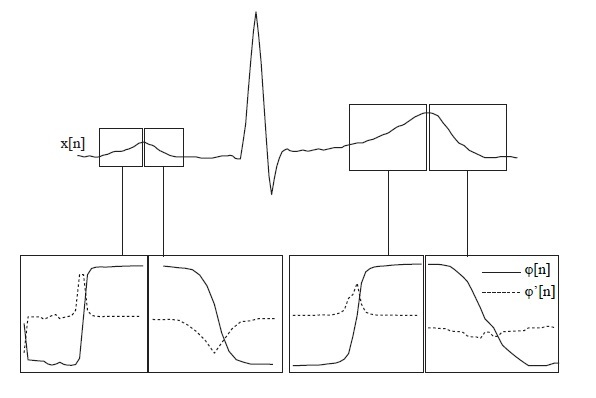
\includegraphics[width=\textwidth,keepaspectratio] {Waves/img/dzialania_fazowej.jpg}
\caption{Zależność między fazą $\phi$ a badanym sygnałem EKG. Źródło: \cite{Waves_aNMfADoEFPBotPT}  }
\label{fig:Waves_DzialFaz}
\end{figure}

Dzięki tej transformacji można odwzorować niewielką amplitudę fali P w funkcję arcustangens zawierającym wartości z przedziału [-pi/2,pi/2], co ułatwia jej wykrycie. Wykrywanie fali P za pomocą tego algorytmu polega najpierw na znalezieniu maksimum lokalnego fali P (P-middle), a następnie dokonania niezależnego wykrycia początku i końca fali (P-onset i P-end). Schematy blokowe wykrycia punktów P-middle i P-onset (P-end jest analogiczny) są zamieszczone na rysunkach ~\ref{fig:Waves_SchemPMid} oraz ~\ref{fig:Waves_SchemPOnset}

\begin{figure}[h!]
\centering
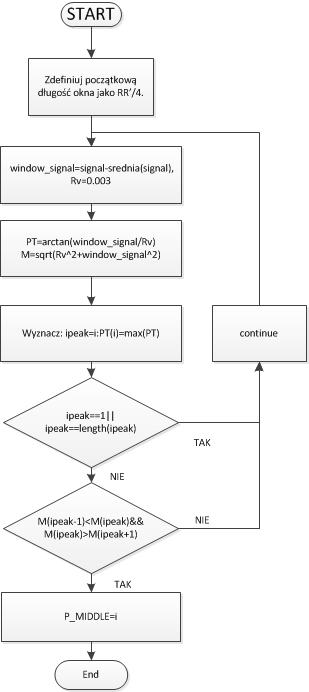
\includegraphics[scale=0.8] {Waves/img/schemat_Pmiddle.jpg}
\caption{Schemat blokowy algorytmu wykrywającego P-MIDDLE  }
\label{fig:Waves_SchemPMid}
\end{figure}

\begin{figure}[!h]
\centering
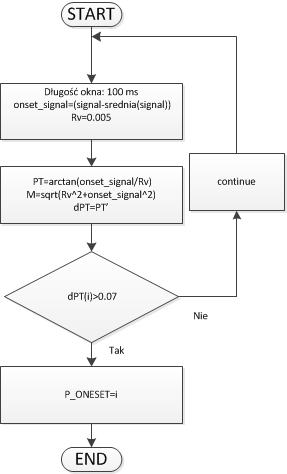
\includegraphics[scale=0.8] {Waves/img/schemat_P_oneset.jpg}
\caption{Schemat blokowy algorytmu wykrywającego P-ONSET (dla P-END jest podobny)  }
\label{fig:Waves_SchemPOnset}
\end{figure}

\subsection{Rezultaty i wnioski}
Ewentualne użycie oprogramowania do detekcji zespołów QRS w urządzeniach medycznych wymaga dokładnego testowania i oceny skuteczności. Zgodnie z literaturą \cite{Waves_TPoSQD} działanie algorytmów ocenia się na podstawie dwóch parametrów: czułości - $S_e$ (ang. sensitivity) i poprawnej wykrywalności - +P (ang positive predictivity). Wskaźniki te definiuje się odpowiednio jako ~\ref{eq:Waves_Se}, ~\ref{eq:Waves_plusP}:

\begin{equation} \label{eq:Waves_Se}
S_e=\frac{TP}{TP+FN}
\end{equation}
oraz
\begin{equation} \label{eq:Waves_plusP}
+P=\frac{TP}{TP+FP}
\end{equation}
gdzie: \newline
TP - (ang. true positive) ilość próbek wykrytych poprawnie \newline
FP - (ang. false positive) ilość próbek wykrytych błędnie \newline
FN - (ang. false negative) ilość zespołów QRS dla których algorytm nie zwrócił wyników \newline
Implementacja algorytmu zespołu QRS wyklucza możliwość występowania FN, dla każdego wejściowego załamka R zawsze zwraca parę punktów oznaczających QRS-onset o QRS-end. W związku z tym czułość algorytmu zawsze wynosi jeden. Inaczej jest dla algorytmu detekcji fali P. Ponieważ jak pisano wcześniej fala P może być przysłonięta, algorytm najpierw dokonuje oceny czy fala P istnieje. Jeśli stwierdzi brak fali P naturalnie nie wyznacza jej punktów charakterystycznych. W takiej sytuacji może zaistnieć FN, w przypadku gdy algorytm pominie  faktycznie istniejącą falę P. Dlatego, w tym przypadku wyznaczane będą oba wskaźniki. Ponadto algorytm bazuje na wartości interwału pomiędzy kolejnymi załamkami R, dlatego zwraca jedną parę mniej wykrytych początków i końców fali P niż podano wejściowych załamków R. W związku z powyższym konieczne jest też podanie kolejnych R-peaków, bez przerw. Założenie to nie jest spełnione dla wszystkich adnotacji z wykorzystanej bazy referencyjnej, dlatego do testów tego algorytmu brano tylko część adnotacji do pierwszej przerwy.   
Testy przeprowadzono wykorzystując sygnały z bazy QT database dostępnej na stronie http://physionet.org. Baza ta zawiera sto-pięć piętnastominutowych sygnałów z zaznaczonymi przez ekspertów punktami charakterystycznymi dla zespołu QRS, fali P, T oraz U. W każdym sygnale zostało oznaczone co najmniej 30 cykli. Szczegółowy opis bazy danych odnaleźć można w pracy \cite{Waves_aDfEoAfMoQaOWIitE}. Na potrzeby testów, w celu uniknięcia propagacji błędów z innych modułów wykorzystano referencyjne położenia załamków R jako daną wejściową. Wartości wskaźnika poprawnej wykrywalności (+P), a w przypadku fali P także czułości ($S_e$) zebrano w tabeli ~\ref{tab:Waves_tabela1} oraz tabeli ~\ref{tab:Waves_tabela2} .

\begin{table}[h!]
\caption{Wyniki algorytmu poszukującego QRS-onset i QRS-end}
\label{tab:Waves_tabela1}
\begin{tabularx}{\textwidth}{|c|X|X|X|X|X|}
  \hline
sygnał &
ilość cykli  &
TP $QRS_{onset}$ &
TP \hspace{2mm}  $   QRS_{end}$ &
+P $QRS_{onset}$  &
+P \hspace{2mm} $  QRS_{end}$  \\
\hline
sel100 & 30 & 29 & 30 & 96,67 & 100,00 \\
sel103 &
30  &
29  &
29  &
96,67 &
96,67 \\
sel114 &
50 &
37 &
47 &
74,00 &
90,00 \\
sel116 &
50 &
45 &
49 &
90,00 &
98,00 \\
sel117 &
30 &
30 &
28 &
100,00 &
93,33 \\
sel123 &
30 &
29 &
28 &
96,67 &
93,33 \\
sel213 &
30 &
24 &
25 &
80,00 &
83,33 \\
sel223 &
31 &
29 &
29 &
 93,55 &
93,55 \\
sel230 &
50 &
37 &
50 &
74,00 &
100,00 \\
sel231 &
50 &
50 &
47 &
100,00 &
94,00 \\
sel233 &
30 &
29 &
28 &
96,67 &
93,33 \\
sel803 &
30 &
27 &
29 &
90,00 &
96,67 \\
sel808 &
30 &
30 &
29 &
100,00 &
96,67 \\
sel811 &
30 &
27 &
29 &
90,00 &
96,67 \\
sel820 &
30 &
30 &
29 &
100,00 &
96,67 \\
\hline \hline
\multicolumn{4}{|r|}{średnia:}   &
 92,00 &
96,40 \\
\hline

\end{tabularx}
\end{table}

\begin{table}[!h]
\caption{Wyniki algorytmu poszukującego QRS-onset i QRS-end}
\label{tab:Waves_tabela2}
\begin{tabularx}{\textwidth}{|c|p{0.8cm}|X|X|X|p{0.7cm}|p{0.8cm}|p{0.8cm}|X|X|}
\hline
sygnał &
ilość  cykli &
TP $P_{onset}$ &
TP $P_{end}$ &
FN $P_{onset}$ &
FN $P_{end}$&
 $S_e$ $P_{onset}$ &
 $S_e$ $P_{end}$ &
+P  $P_{onset}$  &
+P  $P_{end}$ \\
\hline
sel100 &
29 &
26 &
29 &
0 &
0 &
100,00 &
100,00 &
89,66 &
100,00 \\
sel103 &
29 &
29 &
24 &
0 &
0 &
100,00 &
100,00 &
100,00  &
80,76 \\
sel114 &
29 &
18 &
23 &
2 &
2 &
90,00 &
92,00 &
66,67  &
85,19 \\
sel116 &
49 &
30 &
31 &
0 &
0 &
100,00 &
100,00 &
61,22  &
63,27 \\
sel117 &
29 &
20 &
21 &
0 &
0 &
100,00 &
100,00 &
68,97  &
72,41 \\
sel123 &
29 &
21 &
22 &
0 &
0 &
100,00 &
100,00 &
72,41  &
75,86 \\
sel213 &
29 &
3 &
20 &
0 &
0 &
100,00 &
100,00 &
10,34  &
68,97 \\
sel223 &
30 &
29 &
27 &
0 &
0 &
100,00 &
100,00 &
96,67  &
90,00 \\
sel230 &
33 &
13 &
12 &
20 &
20 &
39,39 &
37,5 &
100,00 &
92,31 \\
sel231 &
49 &
41 &
47 &
0 &
0 &
100,00 &
100,00 &
83,67  &
95,92 \\
sel233 &
29 &
15 &
14 &
0 &
0 &
100,00 &
100,00 &
51,72  &
48,28 \\
sel803 &
29 &
24 &
26 &
0 &
0 &
100,00 &
100,00 &
82,76  &
89,66 \\
sel808 &
29 &
10 &
28 &
0 &
0 &
100,00 &
100,00 &
34,48  &
96,55 \\
sel811 &
29 &
23 &
28 &
0 &
0 &
100,00 &
100,00 &
79,31  &
96,55 \\
sel820 &
27 &
21 &
24 &
1 &
1 &
95,45 &
96,00 &
77,78  &
88,89 \\
\hline \hline
\multicolumn{6}{|r|}{średnia:}   &
94,99 &
95,03 &
71,71 &
82,97 \\
\hline

\end{tabularx}
\end{table}

Jak pokazuje tabela ~\ref{tab:Waves_tabela1} algorytm detekcji punktów charakterystycznych zespołu QRS działa z zadowalającą dokładnością. Świadczy to o poprawności implementacji algorytmu w stworzonym module. Przykładowe działanie algorytmu detekcji punktów QRS-onset i QRS-end dla sygnału sel100 pokazano na rysunku ~\ref{fig:Waves_sel100}.

\begin{figure}[h!]
\centering
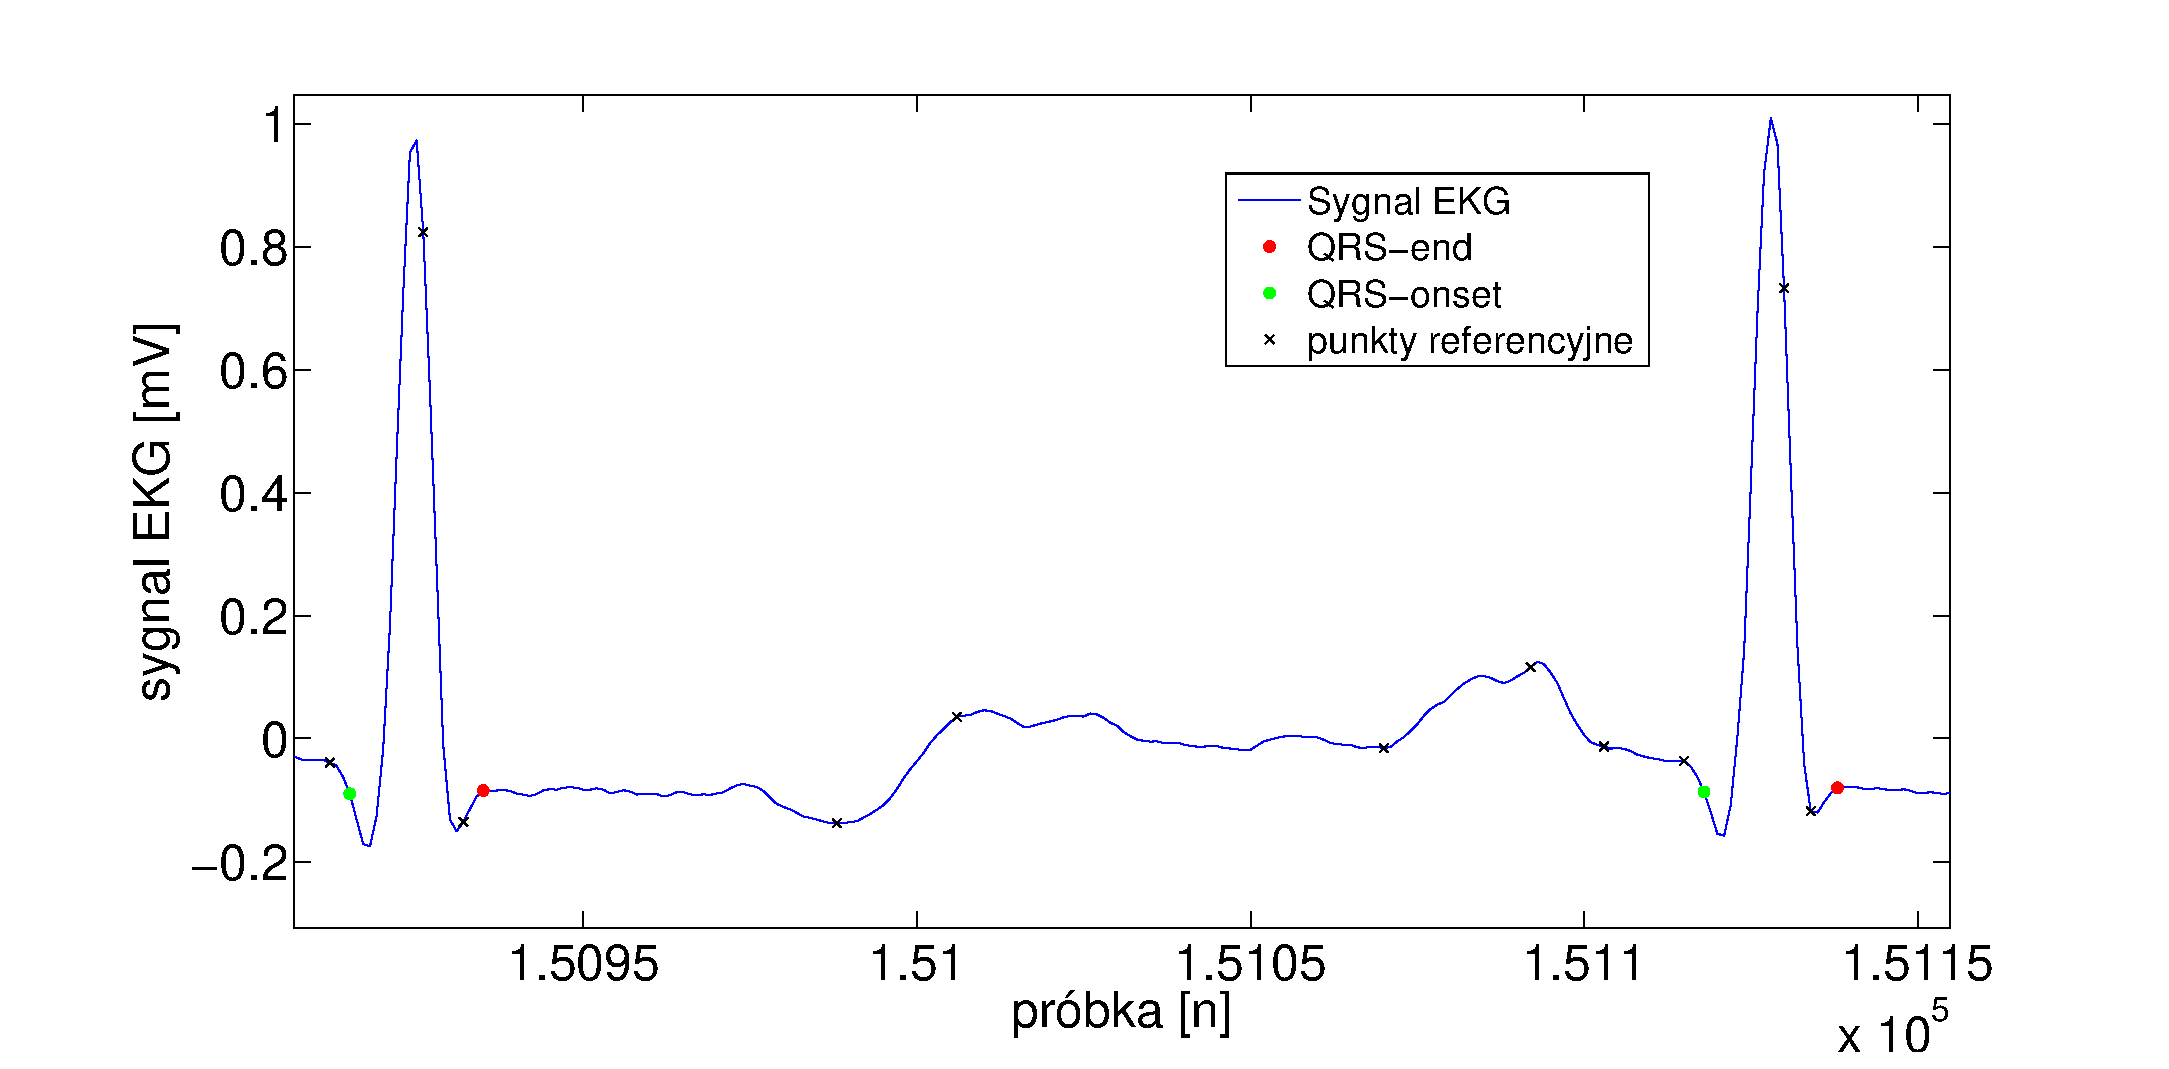
\includegraphics[width=\textwidth,keepaspectratio] {Waves/img/sel100.eps}
\caption{Sygnał sel100 z bazy QT-Database}
\label{fig:Waves_sel100}
\end{figure}

Rysunek ~\ref{fig:Waves_sel100} pokazuje także że jakość dostępnych adnotacji nie jest najlepsza. Punkty oznaczone jako Qrs-end znajdują się na załamkach S, co może spowodować (dla silnie ujemnych wartości załamka S) zaklasyfikowanie poprawnie wykrytego punktu jako błędny.   
Najsłabsze wyniki dla QRS-onset, różniące się o 18\% od średniej, uzyskano dla sygnału sel114. Wyniki +P dla punktu QRS-end nie spadły dla żadnego z testowanych sygnałów poniżej 90\%. Ponownie najsłabiej algorytm poradził sobie z sygnałem sel114, dla którego wynik różnił się od średniej o 6,4\%. Sytuacja taka ma miejsce ze względu na kształt sygnału sel114.
Występuje tam przy załamku R drugi, mający zbliżoną wartość, peak sygnału. Powoduje to zaburzenie kształtu obwiedni, która powinna być funkcją dzwonową obejmującą cały zespół QRS. Skutkuje to błędnym działaniem algorytmu. Sytuację przedstawia rysunek ~\ref{fig:Waves_Error}.

\begin{figure}[h!]
\centering
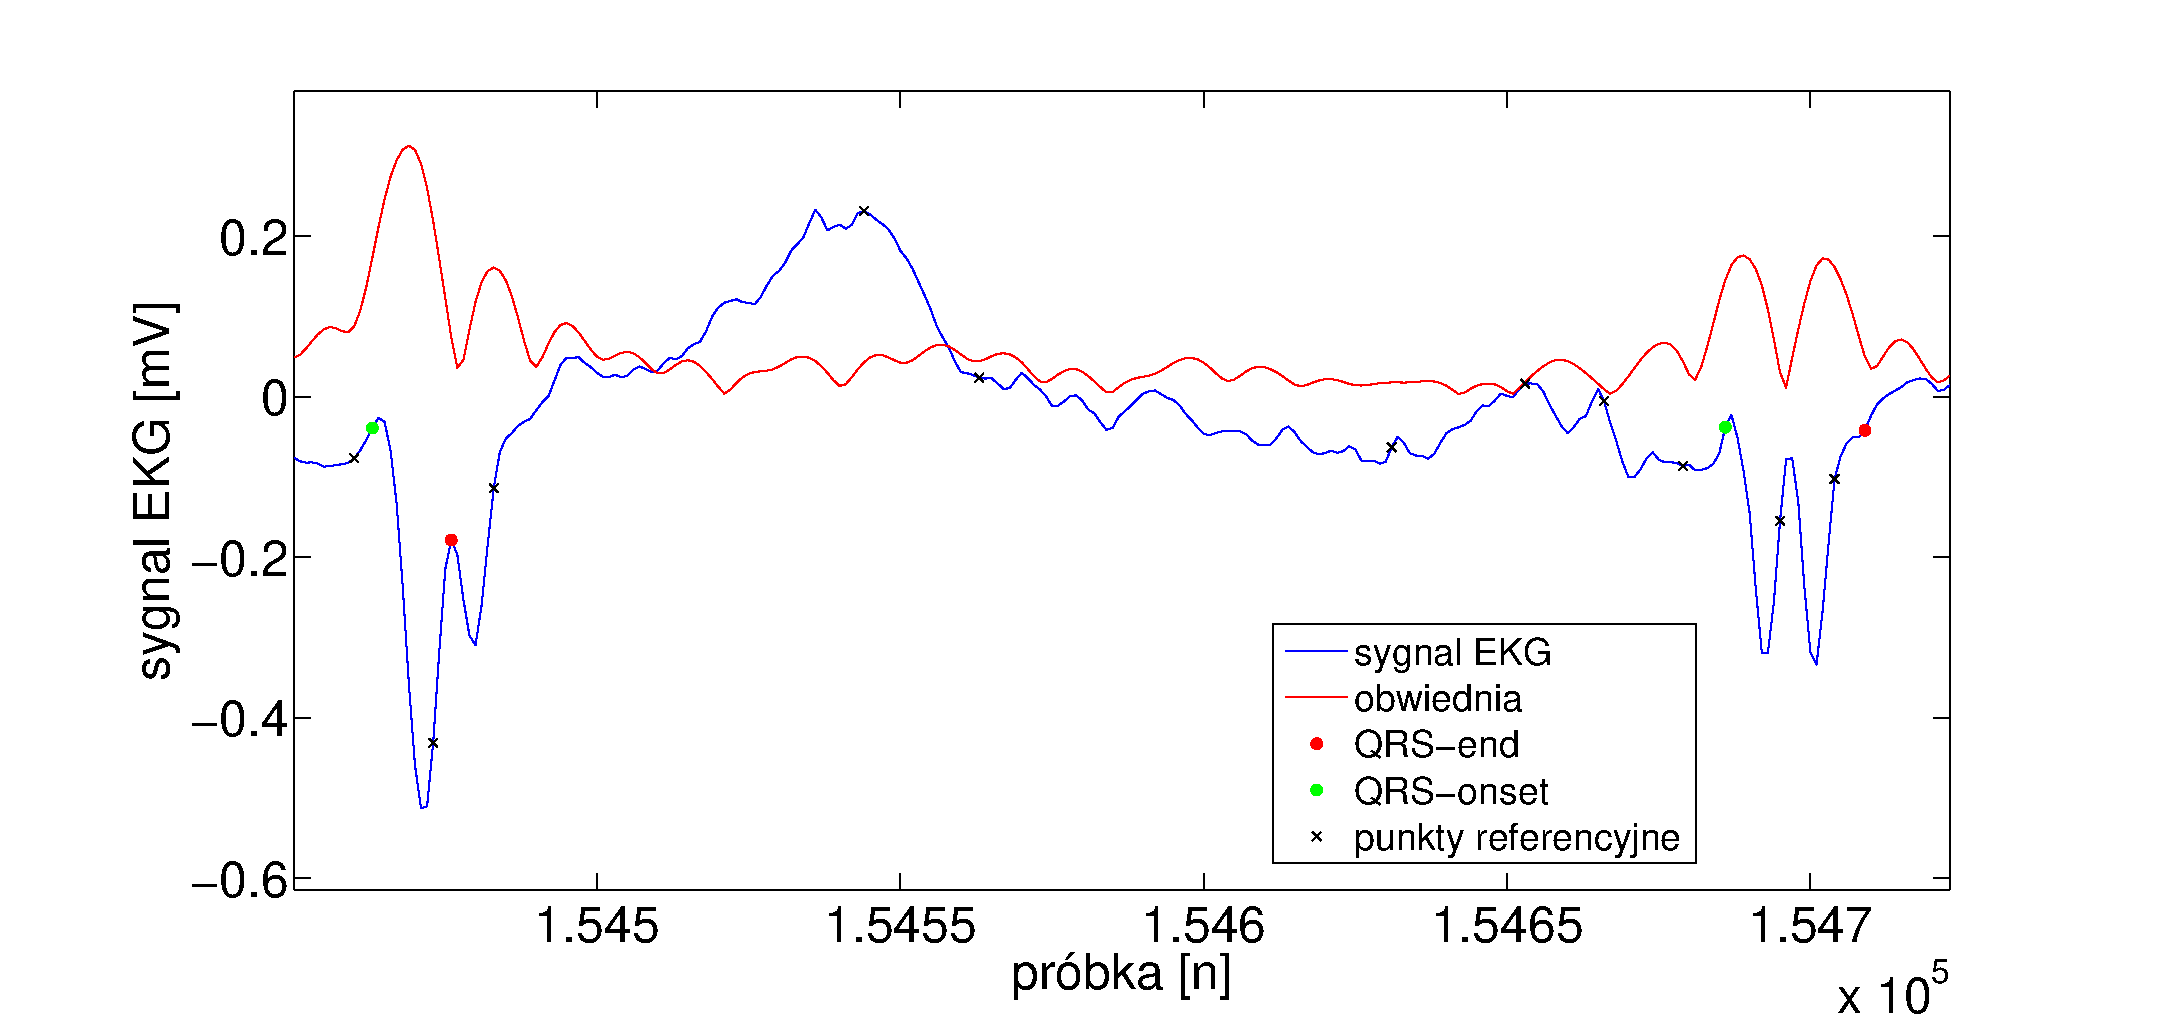
\includegraphics[width=\textwidth,keepaspectratio] {Waves/img/Error.eps}
\caption{Trudny przypadek dla algorytmu detekcji QRS-end oraz QRS-onset}
\label{fig:Waves_Error}
\end{figure}

Jak widać na rysunku ~\ref{fig:Waves_Error}, algorytm dla pierwszego zespołu QRS wykrywa jego koniec w miejscu, w którym ''podwojona obwiednia'' osiąga minimum. W przyszłości błąd ten można by rozwiązać badając czy obwiednia ma dwa maksima lokalne. Jeśli tak należy poszukiwać końca ''drugiej części'' obwiedni.

W przypadku fali P czułość algorytmu jest zadowalająca, choć zdarzają się rekordy, gdzie spada ona poniżej 50\% (według tabeli ~\ref{tab:Waves_tabela2}). Gorzej jest natomiast z wykrywalnością: średnio 71\% dla fali P-ONSET i prawie 83\% procent dla fali P-END. Dzieje się tak wskutek odbiegającego od oryginału kształtu załamka P. W badanych sygnałach bardzo często fala P przyjmowała kształt przedstawiony na rysunku ~\ref{fig:Waves_PrzykP}:

\begin{figure}[h!]
\centering
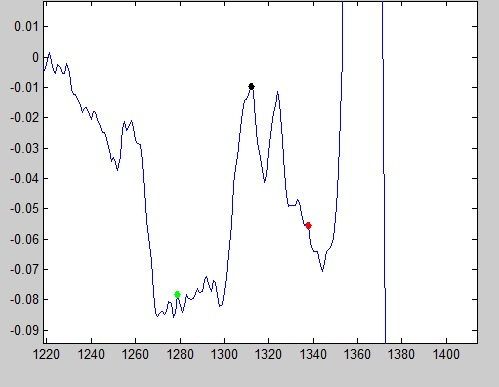
\includegraphics[width=\textwidth,keepaspectratio] {Waves/img/przykladowy_P.jpg}
\caption{Przykładowy załamek P z oznaczonym początkiem P-ONSET (kolor zielony), maksimum P-MIDDLE (kolor czarny) oraz końcem P-END(kolor czerwony).  }
\label{fig:Waves_PrzykP}
\end{figure}

Problem tkwi w położeniu P-MIDDLE; gdy znajduje się on zaraz na początku fali lub na jej końcu, okno (o długości 100 ms) łapie za długi odcinek sygnału leżący poza falą P i na niej może znaleźć nieprawidłowe punkty. Takie sytuacje, jak się okazało w badanych sygnałach zdarzają się bardzo często, dlatego też często punkty nie zgadzają się z punktami naniesionymi przez ekspertów. Problem nie jest łatwy do rozwiązania, gdyż stawiając ostrzejszy warunek na pochodną fazy otrzymujemy punkty P-ONSET i P-END na fali P, ale są one wtedy zbyt późne (dla początku) i zbyt wczesne dla (dla końca) w stosunku do wartości referencyjnych, więc mimo optycznego polepszenia sytuacji (wykryte punkty nie wypadają poza falę P), wykrywalność algorytmu staje się gorsza (gdyż przyjmuje się, że punkt został wykryty prawidłowo, gdy między nim a wartością referencyjną występuje maks 5 próbek różnicy. 
Doświadczenia pokazały,że algorytm w postaci proponowanej w publikacji \cite{Waves_aNMfADoEFPBotPT} może być zastosowany jedynie do zgrubnej detekcji granic fali P, gdyż nie jest wystarczająco dokładny i dla bardzo zniekształconej fali P daje słabe rezultaty. Aby zwiększyć jego wykrywalność, należało by może  wprowadzić zmienną długość okna po wykryciu punktu P-middle w zależności od zaistniałej sytuacji  lub też po wykryciu tego punktu zastosować inny algorytm.